\documentclass[pdftex,11pt,letterpaper]{article}

\setlength{\parskip}{7.2pt}
\setlength{\parindent}{0pt}

\usepackage{fullpage}

\usepackage{float}
\usepackage{graphicx}
\usepackage{amsmath}

\usepackage{hyperref}
\hypersetup{pdfauthor={Silas Baronda},%
            pdftitle={Scarlet Installation \& Configuration Guide},%
            colorlinks}
\urlstyle{same}

\usepackage{draftwatermark}
\SetWatermarkAngle{45}
\SetWatermarkLightness{0.8}
\SetWatermarkFontSize{5cm}
\SetWatermarkScale{4}
%\SetWatermarkText{CONFIDENTIAL}

\begin{document}

\title{Scarlet Installation \& Configuration Guide}
\author{Silas Baronda\\\href{mailto:barondas@cse.ohio-state.edu}{barondas@cse.ohio-state.edu}}

\date{\today}
\maketitle

\tableofcontents
\newpage

\listoffigures
\newpage

\section{Introduction}

Scarlet is an application used by the \href{http://biology.osu.edu/}{Center for Life Sciences Education} to assist with various tasks, such as processing exams, administering workshops, documenting TA progress, and administering ACS surveys.

Scarlet has many different features that you choose from when configuring.

\begin{itemize}
\item a TA database
\item TA FAQs
\item Courses
\item Textbooks
\item Workshops
\item Surveys
\end{itemize}

For this installation guide we are only supporting the use of Surveys.

\subsection{Intended Audience}

The intended audience a System Administrator that is familiar with using virtual machines in particular VirtualBox and the OVA file format.  With that said, you can install Scarlet on your own computer but will require a System Administrator to finish.

Note:
At OSU Biology we use Xen servers for hosting our applications and VirtualBox for any desktop development.  We also recommend VirtualBox for any one-off installations of Scarlet.

Note:
\textit{.ova} format does not require you to use VirtualBox and is not exclusive to VirtualBox.  The \textit{.ova} format is an industry standard that should be supported by any enterprise virtualization software available after September 2007.  If your virtualization software does not support \textit{.ova} format then you need to contact your virtualization software vendor for assistance.  This documentation is a written guide to installing Scarlet on VirtualBox.

\subsection{Requirements}

\begin{itemize}
\item VirtualBox 4.0.4 or greater
\item a statically assigned public IP address 
\item port 80 to be opened to and from the Internet
\item domain name to point to this public interface
\end{itemize}

Note:
The server acquires its IP address via a DHCP server.  You can assign a static IP address via the MAC address for a DHCP server.  The MAC address for a VirtualBox appliance can be found in the Networking Settings for the appliance. You will need to provide the appliance's MAC address to your network administrator to always get the same IP address.

\subsection{Time Required}

On a modern computer, (less than two years old), installation should take at most two hours to install.

If you choose to setup a domain name, please know that DNS Propagation might take up to 48 hours.

\section{Installing Scarlet}

These next sections will take you through the process or installing Scarlet on your system.

\subsection{Requirements}

Because Scarlet was built inside VirtualBox virtualization software, you will need to first download this software.  Scarlet is most compatible with VirtualBox but should work in other virtualization software.
\footnote{Scarlet was exported from VirtualBox in a \textit{.ova} file.  This file should be compatible with other software that can convert \textit{.ova}.}

\subsection{Downloading}

We need to download two files before we can begin, the virtualization software and appliance, Scarlet.

\begin{enumerate}
  \item Download VirtualBox from: \url{http://virtualbox.org}
  \item Download Scarlet from: \url{http://opensource.osu.edu/~barondas/scarlet/scarlet-LATEST.zip}
\end{enumerate}

\subsection{Installing}

After you have installed VirtualBox, you are ready to install Scarlet.

\begin{enumerate}
  \item Install VirtualBox via the directions on the \url{http://virtualbox.org} homepage.
\item Unzip the download Scarlet appliance.
\item Start VirtualBox to launch the VirtualBox Manager as shown in Figure \ref{fig:virtualbox_manager}.  This window shows a list of all the appliances that are installed on your system.

  \begin{figure}[H]
    \begin{center}
      \leavevmode
      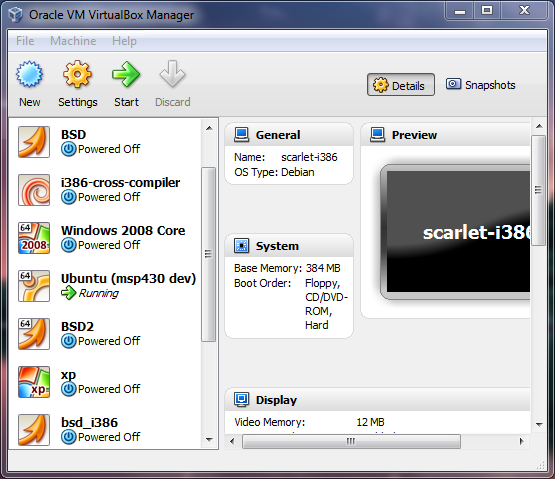
\includegraphics[]{scarlet_images/virtual_box.png}
    \end{center}
    \caption{VirtualBox Manager}
    \label{fig:virtualbox_manager}
  \end{figure}

\item Import the Scarlet Appliance that you downloaded and unzipped from before.  \textit{File $\rightarrow$ Import Appliance}.  You should see something similar \ref{fig:import_wizard_1}.

    \begin{figure}[H]
        \begin{center}
        \leavevmode
            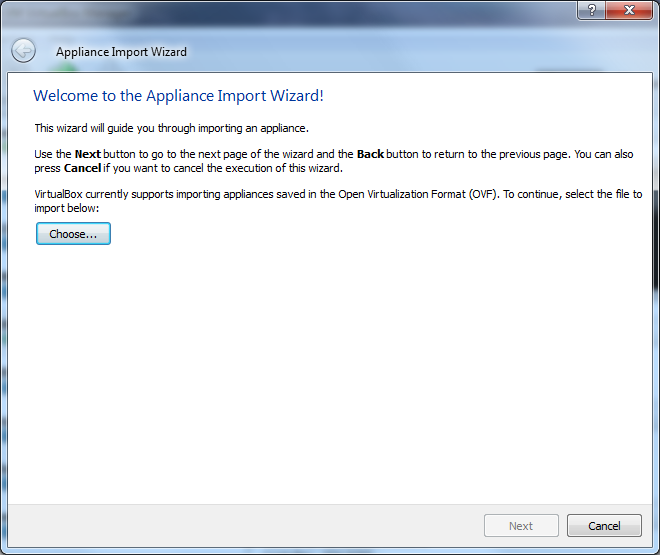
\includegraphics[]{scarlet_images/import_wizard_1.png}
        \end{center}
        \caption{Importing VirtualBox Appliance step 1.}
        \label{fig:import_wizard_1}
    \end{figure}
    
\item Click \textit{Choose}

\item Navigate to the folder that you unzipped the \textit{.ova} file.

    \begin{figure}[H]
        \begin{center}
        \leavevmode
            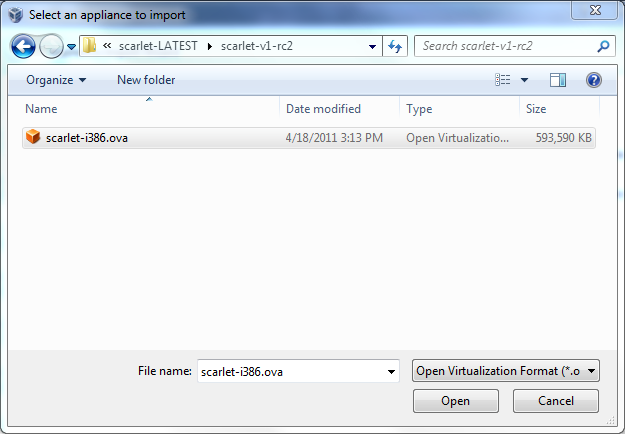
\includegraphics[]{scarlet_images/scarlet_ova.png}
        \end{center}
        \caption{Importing VirtualBox Appliance step 2.}
        \label{fig:import_wizard_2}
    \end{figure}
    
\item Click \textit{Next} You should see a screen as shown below.  Don't change anything and just click \textit{Finish}.

    \begin{figure}[H]
        \begin{center}
        \leavevmode
            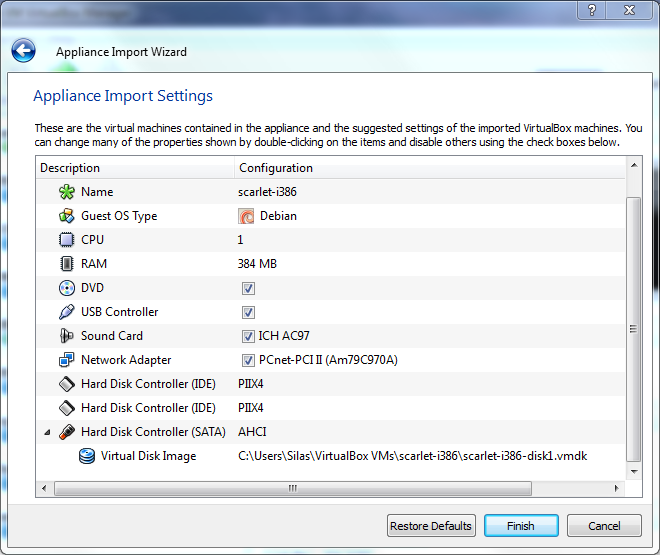
\includegraphics[]{scarlet_images/import_wizard_3.png}
        \end{center}
        \caption{Importing VirtualBox Appliance step 3.}
        \label{fig:import_wizard_3}
    \end{figure}
    
\item It should start importing the appliance.  You should get a screen similar to shown below.

    \begin{figure}[H]
        \begin{center}
        \leavevmode
            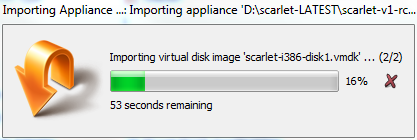
\includegraphics[]{scarlet_images/import_wizard_4.png}
        \end{center}
        \caption{Importing VirtualBox Appliance step 4.}
        \label{fig:import_wizard_4}
    \end{figure}
    
\item After it imports you should now have a Scarlet appliance in your \textit{VirtualBox Manager window}.  It should be called \textit{scarlet-i386}.

    \begin{figure}[H]
        \begin{center}
        \leavevmode
            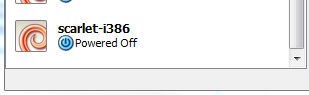
\includegraphics[]{scarlet_images/scarlet_finished_importing.png}
        \end{center}
        \caption{Scarlet done being installed}
        \label{fig:scarlet_finished_importing}
    \end{figure}

\end{enumerate}

This concludes installing \textit{Scarlet}. The next section takes you through configuring the network.

\section{Configuration}
\label{sec:configuration}

After installation we need to configure the networking of the appliance.  There are four types of networking but we will only be covering bridged networks since it gives an public IP easily.

\begin{enumerate}

\item Open the \textit{VirtualBox Manager}.
\item Choose \textit{scarlet-i386}
\item Single Click \textit{Settings} button as shown below.

    \begin{figure}[H]
        \begin{center}
        \leavevmode
            
\includegraphics[]{scarlet_images/settings_button.png}
        \end{center}
        \caption{Settings Button}
        \label{fig:settings_button}
    \end{figure}
    
\item Click \textit{Network Settings} and you should see something similar to below.

    \begin{figure}[H]
        \begin{center}
        \leavevmode
            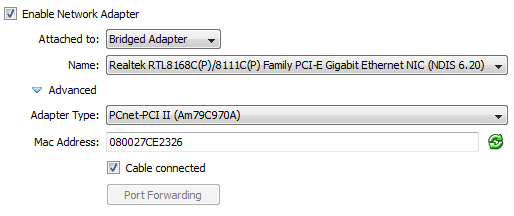
\includegraphics[]{scarlet_images/network_settings.png}
        \end{center}
        \caption{Network Settings}
        \label{fig:network_settings}
    \end{figure}
    
\item There is a bug in the \textit{VirtualBox} when importing an appliance with a bridged network.  To fix this select the \textit{Name:} drop down list for the current network adapter and choose the same network device.

\item Click \textit{OK}

\end{enumerate}

This concludes configuring \textit{Scarlet}. The next section will take you through starting up \textit{Scarlet}.

\section{Starting up}

Staring up \textit{Scarlet} is simple.

\begin{enumerate}

\item Open \textit{VirtualBox Manager} and single click the \textit{scarlet-i386}.

\item Click the \textit{Start} button.  It should look similar to the picture below.

    \begin{figure}[H]
        \begin{center}
        \leavevmode
            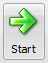
\includegraphics[]{scarlet_images/start_button.png}
        \end{center}
        \caption{Start Button}
        \label{fig:start_button}
    \end{figure}
    
\item A window will open and \textit{Scarlet} will start booting up.

\item After it is finished booting (after all the text stops scrolling). You should find the public IP address towards the bottom of the window.  It will say ``\textbf{Your IP is 10.0.1.106}'' or if something is mis-configured ``\textbf{Your IP is NIL}''.

    \begin{figure}[H]
        \begin{center}
        \leavevmode
            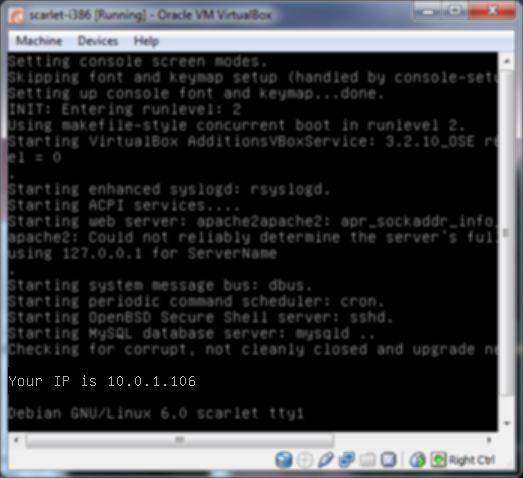
\includegraphics[]{scarlet_images/scarlet_running_blurred.png}
        \end{center}
        \caption{Scarlet Running}
        \label{fig:scarlet_running}
    \end{figure}

\end{enumerate}

This concludes the document \emph{Scarlet Installation \& Configuration Guide}.  If you have ran into any errors please look at the section~\ref{sec:troubleshooting} on page~\pageref{sec:troubleshooting}.

\section{Troubleshooting}
\label{sec:troubleshooting}

\subsection{Nonexistent host networking interface, name 'br0'}

Upon booting up \textit{Scarlet} you may encounter a \verb+Nonexistent host networking interface, name 'br0'+.

    \begin{figure}[H]
        \begin{center}
        \leavevmode
            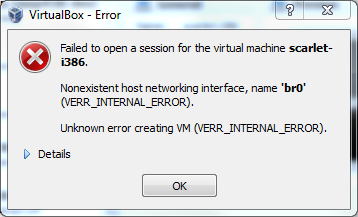
\includegraphics[]{scarlet_images/network_error.png}
        \end{center}
        \caption{\emph{Nonexistent host networking interface, name `\textbf{br0}'}}
        \label{fig:network_error}
    \end{figure}
    
To fix this complete the steps listed in section~\ref{sec:configuration} on page~\pageref{sec:configuration}.


\end{document}

